\capitulo{5}{Aspectos relevantes del desarrollo del proyecto}
En este punto de la memoria haremos un repaso de los puntos más importantes del desarrollo del proyecto, se comentarán aspectos relacionados con todo lo visto anteriormente, y dividiré este apartado en 3 partes diferenciadas: El comienzo, el desarrollo con realidad virtual y una final sobre el trabajo con la robótica\cite{Robotica}.

\section{Comienzo del proyecto}
Como no podría ser de otra manera a lo largo de la primera semana, me dediqué junto a mi tutor a la toma de decisiones en referencia a lo que ibamos a hacer, planificación de tareas y la metodología a seguir en cuanto a la forma de trabajar. 

Desde ya antes de comenzar mi etapa en ITCL cuando dimos por hecha mi incorporación al departamento, yo comencé a aprender desde las cosas más básicas de Unity hasta algunos conceptos ya más complicados gracias a un curso de desarrollo con Unity que me compartió mi tutor. Cuando fue terminada la parte de planificación yo me encargué de seguir el curso, con un ímpetu especial en aquellas partes que estaban muy relacionadas con nuestras tareas. 

Por otra parte empecé a manipular las Oculus Quest 2 \cite{Quest2} con el motivo de conocer un poco más un dispositivo del que únicamente había oído hablar pero que nunca había utilizado. El ver sus interfaces, el manejo de los controles, la manera de seguir las manos o probar experiencias interactivas me ayudaron a entender qué era el dispositivo con el que iba a trabajar. Al igual que con este dispositivo me dediqué también al uso de los guantes Nova\cite{SGloveNova} con previa lectura del manual de usuario que contenían. Para probar a nivel usuario estos guantes, me enfrenté con unas escenas de prueba desarrolladas en Unity que se encontraban en el plugin de SenseGlove.

\section{Desarrollo con Realidad Virtual}
Esta sección será dividida en dos partes, una en la que veremos la parte del desarrollo primeramente con los guantes y la otra en la que fusionaremos el uso de los dos dispositivos.
\subsection{Trabajo con Nova\cite{SGloveNova}}
A partir de este momento, me adentré en la parte de trabajo real con los guantes y empecé con la que sería la primera tarea: Monitorizar y parametrizar aquello que nos ofrecen estos guantes.   Para ello tuve que bucear entre la documentación que venía con el SDK y ver las clases que tenía, así pudimos ver todo aquello que nos ofrece. Los datos que encontramos que nos ofrecían mayor relevancia, eran aquellos relacionados con las flexiones y posiciones de los dedos, datos de calibración, ángulos de los dedos, vibraciones en cada punto y los que nos mostraban la batería. 

El objetivo en primera instancia era representar en una escena nuestra mano gracias a los guantes y crear un panel de control para aprender a manejar las funcionalidades que estos tienen. Para poder representar los datos comentados, de manera correcta fue necesario desarrollar un script al que le dí el nombre de \textit{GettingData}. Con él recojo estos valores de los sensores y automáticamente se actualizan en un diccionario donde las claves son los nombres de los dedos o el IMU(Unidad de medición inercial, para la rotación de la mano)  y sus valores los obtenidos.

Lo conseguimos, mostrando en la escena junto a una representación tridimensional de la mano un panel de texto. Este refleja en él la posición de los dedos, indicando el nivel de flexión y de abducción(en caso del pulgar), la rotación gracias al IMU(Unidad de medición inercial) que lleva integrado en el reverso de la mano, el nivel de batería del dispositivo(entre 0 y 1) e incluso el nombre del dispositivo conectado. Estableciendo así por fin, la primera conexión a una escena propia para probar y desarrollar.

Gracias a esta escena podemos acceder a algunas de las funciones que nos ofrecen estos guantes. Y es que, a través de unos sliders colocados en el panel, podemos hacer vibrar alguna de las partes de los guantes y probar también el motor de respuesta que lleva integrado para los dedos. Este funcionamiento lo implemento gracias al script de nombre \textit{HapticsManager}. Para cumplir con lo que queríamos, en ese script se crean objetos que el dispositivo toma como comandos para realizar las funciones. Los sliders se enlazan desde el inspector de Unity a cada una de las funciones determinadas.

A continuación muestro una imagen de la escena una vez ejecutada correctamente:
\begin{figure}[h]
\centering
\label{Escena de control de los guantes}
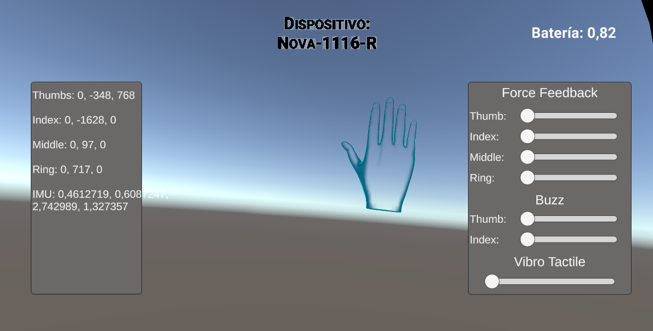
\includegraphics[width=0.9\textwidth]{hapticsmanager.PNG}
\caption{Escena de control de los guantes}
\end{figure}

\subsection{Fusionando Tecnologías}
Llegado a este punto, di un paso más allá en mi camino hacia el desarrollo de VR\cite{VR} con Unity, estableciendo la primera conexión del dispositivo Oculus Quest 2 y sus controladores Touch a una escena desarrollada por mí. Esta escena llamada por mí \textit{oculusTesting}, la utilicé para llevar a cabo algunas pruebas. Aquí trabajamos para ver que nos ofrecían y para que podemos usarlas. 
En este punto enfrentamos algunas complicaciones, ya que era necesario usar los plugins tanto de Oculus como de XR y cambiar algunos ajustes del software para que funcionase correctamente.

Tras las pruebas, gracias a las posibilidades de tracking a partir de la componente Transform\cite{Transform} de Unity pudimos obtener de una manera realista tanto datos de la posición en el espacio como de su rotación, lo cual nos fue útil para poder desarrollar dentro de nuestro proyecto. En este punto el movimiento de la cámara principal se encuentra enlazado al movimiento de nuestra visión desde las gafas, sincronizando así gafas de juego y la visión.

Aquí comencé a realizar una nueva escena, de nombre \textit{GloveAndOculus} donde buscaba adaptar la de diagnóstico y control háptico de los guantes a un uso conjunto con las gafas y controladores, pero cambiando el panel controlador por uno con datos del tracking de Oculus. Para conseguir esta adaptación fue fundamental el cambiar el tipo de interfaz de usuario dentro de la escena para que deje de ser estático en la pantalla (lo que provocaba fallos) y pase a verse desde las gafas Oculus (world space). Una vez conseguido esto, el siguiente paso que buscaremos será el de intentar representar las dos manos(con los guantes) y utilizar los controladores para trackear y establecer de manera real la posición y la rotación de las manos. Habrá que montar los Touch sobre los propios guantes.

Se consiguió el objetivo marcado en una escena llamada \textit{SeeingHands}, pero antes tuve que montar sobre el reverso de los guantes un soporte que contienen dentro del packaging del producto con el uso de unos tornillos que también venían. Fue necesario utilizar el tutorial que tienen en su página para poder montarlo correctamente. Esto es necesario por que al no tener los guantes posibilidad de tracking, montando unos controladores de VR\cite{VR} sobre ellos podemos cubrir esta opción. Tras este montaje, establecí las conexiones de los dispositivos a Unity, y desarrollé un pequeño script donde asignamos la componente\cite{Componentes} transform de los controladores a la del objeto de nuestros guantes(la representación digital de nuestras manos). Con esto y una opción que tiene el objeto de los guantes que permite especificar el tipo de controlador que se está usando, conseguimos que se vean las manos representadas de manera correcta en posición y rotación en el espacio. 

\section{Trabajo con Robótica}
En esta sección veremos el desarrollo y trabajo con el brazo robótico Kinova, lo dividiremos en dos instancias, una en la que trabajamos de manera simulada con una replicación virtual y otra, de manera real.
\subsection{Trabajo sobre Simulación}
Llegados a este punto lo que queríamos era llevar a cabo la replicación virtual de lo que sería el robot real. Para ello utilizamos un diseño de una pinza robótica hecha por nuestros compañeros dentro de esta escena. Las funciones que ejecturía el brazo realmente son la de desplazamiento en el espacio y la apertura/cierre de la pinza. A través de un script de nombre \textit{VirtualRobot} se implementaron los métodos get y set de la posición en las tres dimensiones del espacio y de la apertura de esta pinza para poder abrirla y cerrarla. En este apartado tuve complicaciones, que se solventaron profundizando en el estudio de la documentación de Unity centrándome en la parte de rotation y sus valores/tipos de datos de la componente Trnasform. Utilizo una variable de nombre \textit{Apertura} que unifica la rotación de la componente X de cada brazo de la pinza de manera que se muevan simultáneamente, simulando el movimiento real de abrir y cerrar la pinza. 
\begin{figure}[h]
\centering
\label{Cierre y apertura total de la pinza robótica}
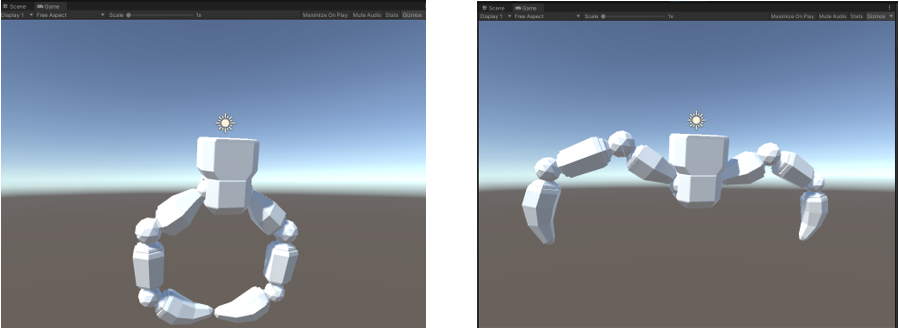
\includegraphics[width=0.9\textwidth]{img/pinza open close.PNG}
\caption{Cierre y apertura total de la pinza robótica}
\end{figure}
 Posteriormente la escena de replicación virtual de la pinza del robot fue mejorada implementándose dentro del script además de los getters y setters, dos métodos de movimiento. El primero de ellos en el espacio, dada una velocidad lineal y una posición objetivo, se mueve desde su origen hasta allí con esa velocidad. También se implementó el segundo, que controla el movimiento de apertura de la pinza, también dada una velocidad para la apertura y seleccionando una apertura objetivo. 
 
 El siguiente paso era hacer funcionar la pinza y desplazarla con nuestras manos, para ello creé una nueva escena en la que unimos la parte desarrollada para poder tener nuestras manos representadas en el espacio en tres dimensiones y con sus movimientos, junto con lo desarrollado para la pinza del robot. Para conseguirlo ha sido desarrollado el script \textit{Connector} el cual se encarga de hacer de puente de conexión entre guantes y la pinza. La lógica que se ha aplicado es que la pinza siga el desplazamiento de la mano gracias a la función de movimiento y la velocidad fijada, pero a una posición cercana para poder tener ambas cosas en vista. Además, ha sido implementada la idea de que al hacer con nuestros guantes el gesto de cerrar índice y pulgar, la pinza simule ese movimiento con la apertura que indiquemos con nuestro guante y a la velocidad de apertura marcada. Esto lo hemos podido conseguir gracias a recoger los datos de las flexiones de los dedos con nuestro script \textit{GettingData} que llevamos a cabo al principio.
 
 \subsection{Trabajo real}
Llegados a este punto, comenzamos con la integración del robot en el proyecto, primero realizamos una serie de pruebas desde otro proyecto en unity y después ya en el propio del TFG donde he creado una nueva escena de nombre \textit{ROSConnector} desde la cual con los scripts nos comunicaremos con nuestro robot. El funcionamiento de la escena es el siguiente:

En primer lugar, un objeto \textit{ROSInitializer} que contiene la componente del script de mismo nombre al que le daremos el dato de la IP del robot, en este caso 192.168.50.103 y el dato de número de puerto, para poder establecer la conexión. Hijos de este objeto, otros dos. Uno será un objeto para probar Kinova al que se le asocia un \textit{ROSInitializer} y el nombre de servicio. Y el otro el controlador Kinova que nos permite mandar instrucciones de desplazamiento tanto angular como linear al brazo y regular la apertura de la pinza. 

En cuanto a la conexión física del robot previa a Unity, utilizamos un router que se encuentra conectado a mi pc y a un switch que a su vez está conectado a la red. Para ello dentro de las opciones de configuración del adaptador de red, en el apartado TCP/IPv4 tenemos que seleccionar manualmente la subred que nos permita comunicarnos con el robot. Gracias a hacer ping y usar el comando \textit{ipconfig} podemos comprobar que todo esté correcto.

Para poder saber, entender y aprender como utilizar el robot entramos dentro de él gracias a establecer la conexión a través del SSH\cite{SSH} a la dirección IP del robot. Hubo que cambiar por medio de Nmtui la opción de asignación red del robot a automática y buscarla por su número de MAC en el escáner de redes. Desde aquí podemos acceder a información del robot y, utilizando el comando \textit{rostopic list} se nos muestra toda la lista de posibles comandos que podemos usar para interactuar con él. Esta lista se cribó para ver cuáles eran útiles para nuestro objetivo.

Finalmente, fuimos a por el último objetivo fusionando todo lo aprendido y desarrollado. La última escena contiene tanto la parte de VR y conexión al dispositivo Oculus y sus controllers, como la conexión a los guantes hápticos y como no, la conexión al robot. El objetivo de esta escena será, finalmente, controlar el robot con nuestro controller Oculus\cite{Quest2} montado sobre el guante, para así mover el brazo robótico en el espacio y cerrar y abrir la pinza solo con tener el guante puesto. 

Para alcanzar el objetivo de esta escena ha sido necesario, a nivel de software, el escribir un Script al que he llamado \textit{BotHandsLinking}. Este script es el manager que gestiona esta escena, ya que permite trabajar sobre el Kinova Position Controller que tenemos desarrollado anteriormente, al que le envía los datos del controller Oculus (referidos a la posición) para mover el brazo en el espacio. Se restringen los valores y se aplican offsets, de cara a una mejor experiencia de usuario. El controlador de posición es un script que publica en un topic los mensajes con las posiciones objetivo en los ejes X Y Z del robot.
Además se controla también la rotación de la mano.

Para finalizar el desarrollo del proyecto de fin de grado, ha sido añadido un script a esta última escena llamado \textit{GripManager} que se encarga de aplicar sobre una componente del robot que se ocupa de publicar los mensajes relacionados con la apertura o cierre de la pinza del robot, la lógica utilizada en las escenas previas. Esta lógica toma los valores recogidos por los guantes en los dedos y aplica el cierre o apertura deseado sobre la pinza del robot.

